\documentclass{article}
\usepackage{listings}
\usepackage{xcolor}
\usepackage{graphicx,authblk}
\usepackage{geometry,bm}
\usepackage{float}
\usepackage{url}
\usepackage{hyperref}
\usepackage{amsmath,amsfonts}
\usepackage{algorithm2e}
\usepackage{tcolorbox}

\def\tcb@proc@counter@auto#1{%
  \newcounter{tcb@cnt@#1}%
  \csxdef{tcb@cnt@#1}{tcb@cnt@#1}%
  \tcb@proc@counter@autoanduse{#1}%
  \ifcsname resetcounteronoverlays\endcsname%<-added
  \resetcounteronoverlays{tcb@cnt@#1}%<-added
  \fi%<-added
}
\makeatother

\newtcolorbox[auto counter]{egsBox}[2][]{%
colback=alg1!10,colframe=alg1!90, center, fonttitle=\bfseries, title=Example~\thetcbcounter: #2,#1}

\newtcolorbox[auto counter]{algBox}[2][]{%
colframe=alg1!80,colback=alg1!10, center, fonttitle=\bfseries, title=Algorithm~\thetcbcounter: #2,#1}

\definecolor{alg1}{rgb}{0.0, 0.46, 1.0}
\definecolor{alg2}{RGB}{9, 166, 75}
\definecolor{alg3}{RGB}{124,198,137}

\definecolor{greenish}{RGB}{4,191,85}
\definecolor{reddish}{RGB}{174,12,48}
\definecolor{blueish}{rgb}{0.0, 0.46, 1.0}
\definecolor{magenta}{RGB}{250, 54, 139}
\hypersetup{
colorlinks   = true, %Colours links instead of ugly boxes
urlcolor     = blueish, %Colour for external hyperlinks
linkcolor    = greenish, %Colour of internal links
citecolor   = magenta %Colour of citations
}

\def\tvec{\vec{\mathbf{t}}}
\def\nvec{\vec{\mathbf{n}}}
\def\th{\hat{\mathbf{t}}}
\def\nh{\hat{\mathbf{n}}}
\def\mh{\hat{\mathbf{m}}}
\def\eh{\hat{\mathbf{e}}}
\def\et{\tilde{\mathbf{e}}}
\def\ehx{\hat{\mathbf{e}}_x}
\def\ehy{\hat{\mathbf{e}}_y}
\def\ehz{\hat{\mathbf{e}}_z}
\def\etx{\tilde{\mathbf{e}}_x}
\def\ety{\tilde{\mathbf{e}}_y}
\def\etz{\tilde{\mathbf{e}}_z}
\def\r{\mathbf{r}}
\def\ib{\mathbf{i}}
\def\q{\mathbf{q}}
\def\p{\mathbf{p}}
\def\rt{\tilde{\mathbf{r}}}
\def\zt{\tilde{z}}
\def\xt{\tilde{x}}
\def\yt{\tilde{y}}
\def\v{\mathbf{v}}
\def\vt{\tilde{\mathbf{v}}}
\def\vts{\tilde{v}}
\def\C{\mathcal{C}}
\def\R{\mathcal{R}}
\def\Rn{\mathbb{R}}
\def\I{\mathbb{I}}
\def\E{\mathbb{E}}
\def\Q{\mathcal{Q}}
\def\T{\mathsf{T}}
\def\d{\text{d}}
\def\C{\mathbb{C}}
\def\c{\textsf{c}}
\def\s{\textsf{s}}
\def\sgp#1{{\sf \textcolor{red}{#1}}}
\def\mr#1{{\textcolor{blue}{#1}}}
\def\S{\mathcal{S}}
\def\uh{\hat{\mathbf{u}}}
\def\vh{\hat{\mathbf{v}}}
\def\nh{\hat{\mathbf{n}}}

\title{Rotations -- from complex numbers to quaternions}
\author{A Mohanraj, and S Ganga Prasath\footnote{\href{emailto:sgangaprasath@smail.iitm.ac.in}{sgangaprasath@smail.iitm.ac.in}} \\
Department of Applied Mechanics and Biomedical Engineering,\\
Indian Institute of Technology Madras, Chennai 600 036.}
\date{}
\setcounter{Maxaffil}{0}
\renewcommand\Affilfont{\itshape\small}
\begin{document}

\maketitle
\begin{abstract}
Rotation is one of the fundamental operations of geometry. It provides a way to transform vectors from one location to another while hinged with respect to a pre-defined axis. In this first part of the two part primer we introduce this simple yet often confusing geometric operation in 2D and 3D. We start with the complex number representation of the rotation operation in 2D and its connection to the standard matrix version. Then we discuss the Euler-angle representation of rotation of vector basis, their extrinsic and intrinsic forms. Ultimately we introduce quaternions, which are the natural extension of complex numbers to 3D. In the process, we also look at Gimbol locking, an intrinsic berrier in Euler-angle represetation. Each concept discussed is explained with a worked out example and a supplemental \href{https://github.com/sgangaprasath/RotationTut/blob/main/Rotations.ipynb}{\texttt{python}--code} that numerically implements these examples.
\end{abstract}


\section{Introduction}
In this two part series, we are interested in understanding the connection between rotation and geometry of curves 3D. In the first part, we develop the notation and the mathematics behind rotations and in the second we will see how it forms the basis for geometry of curves in 3D. Though understanding geometry of 3D curves is our ultimate objective, we take the 2D route to make the concepts approachable before extending them to 3D. Besides its application to 3D curves, rotation has a variety of applications such as in the kinematics and dynamics of rigid bodies in physics (useful in mechanics of machines, robotics, and flight/rocket/satellite trajectories), animation \& graphic design and so on. In this primer, we start with the rotation operation in 2D, its representation using complex numbers and an example by applying it to transform a vector. We then move to rotations in 3D which is considerably complex than its 2D counterpart. In 3D, we introduce rotation about an arbitrary orientation, the ideas of intrinsic and extrinsic rotation of basis vectors and show how to transform between two arbitrary basis vectors. We end with a generalization of complex numbers to 3D i.e. the quaternions and use it to perform rotations. This primer borrows heavily from these \cite{hanson2005visualizing,vince2008geometric,vince2006mathematics} excellent approachable references.

\section{Rotation in 2D}
We will illustrate rotation in 2D with 3 examples: $(a)$ rotation of a vector represented in cartesian coordinate basis, $(b)$ rotation of the coordinate basis vectors (which will become relevant in sec.~\ref{sec:3D}), $(c)$ rotation of a triangle about the origin. We also show that the complex number system provides an intuitive and simple way to perform rotations. Most of what we see in this section is taught in high-school. Nevertheless, we leave it here to ensure completeness.

\subsection{Complex plane representation}\label{sec:comp2d}
A complex number $z \in \C$ is defined as a number of the form $z = a + i b$, where $a, b \in \Rn$, and $i$ is the imaginary unit with the property $i^2 = -1$. Complex numbers can be graphically represented in a cartesian plane with $a$ representing the magnitude along $\ehx$ and $b$ along $\ehy$ with $\eh_{x,y}$ being the unit vectors along $x, y$-axes (see Fig.~\ref{fig:schm2D}$(a)$). This complex number $z$ corresponds to the point with coordinates $(a, b)$.

\subsubsection*{Polar form of complex numbers}
In addition to the rectangular form, complex numbers can also be expressed in polar notation. The complex number $z$ can be written as $z = re^{i\theta} = a + ib$, where $r$ is the magnitude (or modulus) of the complex number with $r>0$ and $\theta$ is the argument (or angle) of the complex number, shown schematically in Fig.~\ref{fig:schm2D}$(a)$, taking values in the range, $\theta \in [ 0, 2\pi]$, measured from the positive real axis. The term $e^{i\theta}$ is defined using Euler's formula:
\[
e^{i\theta} = \cos \theta + i\sin \theta.
\]
This representation is particularly useful for performing rotations in the complex plane. In polar notation, the multiplication of two complex numbers results in the multiplication of their magnitudes and the addition of their angles, thus providing a straightforward geometric interpretation of complex multiplication as rotation and scaling.

\begin{figure}[ht!]
  \centering
  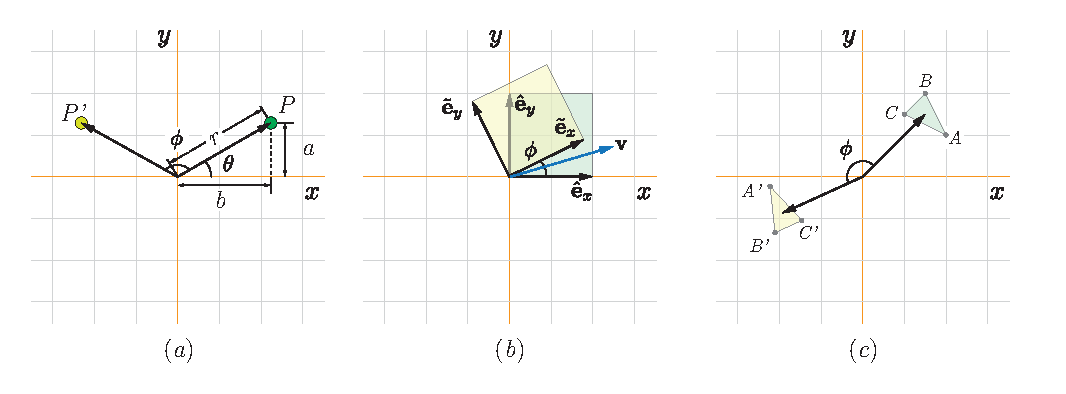
\includegraphics[width=\textwidth]{figs/2Dcomplex.pdf}
  \caption{Schematic showing rotation of 3 different objects in two-dimensions: $(a)$ a vector $P$ located at a distance $r$ and an angle $\theta$ (with $a = r \sin \theta, b = r \cos \theta$) with respect to the origin which when rotated by an angle $\phi$ transforms to $P'$, $(b)$ a coordinate basis, $\ehx, \ehy$ when rotated by an angle $\phi$ transforms to $\etx, \ety$, $(c)$ a triangle $ABC$ when rotated by an angle $\phi$ reaches $A'B'C'$. Refer \texttt{python}-notebook for implementation.}
  \label{fig:schm2D}
\end{figure}

\subsubsection*{Multiplication as rotation and scaling}

When you multiply two complex numbers, you perform a rotation and scaling in the complex plane. The multiplication can be expressed as:
\[
z_1 \cdot z_2 = (a_1 + i b_1)(a_2 + i b_2).
\]
This multiplication changes the magnitude and rotates the point in the complex plane. In polar notation, multiplication of two complex numbers given by, $z_1 = r_1 e^{i\theta_1}$ and $z_2 = r_2 e^{i\theta_2}$, where $r_1$ and $r_2$ are the magnitudes, and $\theta_1$ and $\theta_2$ are the angles of $z_1$ and $z_2$, can be written as,
\begin{equation}
z_1 \cdot z_2 = r_1 e^{i\theta_1} \cdot r_2 e^{i\theta_2} = r_1 r_2 e^{i(\theta_1 + \theta_2)}. \label{eq:compMult}
\end{equation}
This result implies that the magnitudes of the complex numbers are multiplied, and their angles (or arguments) are added. Therefore, multiplication in polar form corresponds to a rotation (given by the sum of angles) and a scaling (given by the product of magnitudes) in the complex plane.

\begin{egsBox}[label={egs:rot2Dex1}, float, floatplacement=t]{Rotating a point using complex number}
  \footnotesize
  Consider a point $P$ represented by the complex number $z = 1 + i\sqrt{3}$ (which corresponds to the point $(1, \sqrt{3})$ in the 2D plane, forming an angle of ${\pi}/{3}$ with the positive real axis). To rotate this point by $120$ degrees (or ${2\pi}/{3}$ radians), we multiply it by $e^{i\frac{2\pi}{3}}$ (which represents a rotation of ${2\pi}/{3}$ radians in the complex plane).
  The multiplication is as follows:
  \[
  z' = z \times e^{i\frac{2\pi}{3}} = (1 + i\sqrt{3}) \times e^{i\frac{2\pi}{3}} = (1 + i\sqrt{3}) \times \left(-\frac{1}{2} + i\frac{\sqrt{3}}{2}\right).
  \]
  Expanding this product, we get:
  \[
  z' = \left(1 \times -\frac{1}{2}\right) + \left(1 \times i\frac{\sqrt{3}}{2}\right) + \left(i\sqrt{3} \times -\frac{1}{2}\right) + \left(i\sqrt{3} \times i\frac{\sqrt{3}}{2}\right) = -\frac{1}{2} - \frac{3}{2} + i\left(\frac{\sqrt{3}}{2} - \frac{\sqrt{3}}{2}\right) = -2.
  \]
  After the rotation, the new position $z'$ of the point $P$ in the complex plane is $-2$, which corresponds to the point $(-2, 0)$ in the 2D plane.
\end{egsBox}

\subsection{Vector components in a rotated frame}\label{sec:VecComp2D}
We briefly move away from the complex plane representation of rotation to the cartesian plane and connect them by the end of this sub-section. Let us consider two basis vectors $\ehx, \ehy$ pointing along $x, y$--axes (see Fig.~\ref{fig:schm2D}$(b)$) which when rotated by an angle $\phi$ in the counter-clockwise direction gives $\etx, \ety$. It is easy to see that $\ehx\cdot\etx=\ehy\cdot\ety=\cos \phi$ and $\ehy\cdot\etx = -\ehx\cdot\ety = \sin \phi$. Now a vector $\v$ with components $\{ v_1, v_2 \}$ in the $\eh_i$ basis transforms to components $\{ \vts_1, \vts_2 \}$ in the rotated basis $\et_i$ i.e., $\v = v_1 \ehx + v_2 \ehy$ and $\vt = \vts_1 \etx + \vts_2 \ety$. A compact way of transforming between these two basis is to write $\v = \Q^\T \vt$ and $\vt = \Q \v$ where $\Q = \{ \etx, \ety \}$ with $\Q$ being the rotation tensor. The rotation tensor $\Q$ can be written explicitly as
\[
  \Q  = \begin{pmatrix} 
  \etx \cdot \ehx & \etx \cdot \ehy \\
  \ety \cdot \ehx & \ety\cdot \ehy
  \end{pmatrix} = 
  \begin{pmatrix} 
  \cos \phi & \sin \phi \\
  -\sin \phi & \cos \phi 
  \end{pmatrix}.
\]

\noindent This matrix $\Q$ is indeed the transpose of the standard rotation matrix $\R$ i.e., $\Q = \R^\T$ for a counter-clockwise rotation, confirming that rotating the basis $\eh_i$ by a counter-clockwise angle of $\phi$ rotates the vector $\v$ by a clockwise angle $\phi$ in the transformed frame $\et_i$. This rotation tensor, $\Q$ is fundamental to what we will see in the second part of the primer. We hope you are holding your breath for the arrival of part 2.

\subsubsection*{Rotation in complex plane vs cartesian plane}
We can express a complex number $z = re^{i\theta}$ in cartesian coordinates as vector $\r = \{ x, y\}$ with $x = r\cos\theta$ and $y = r\sin\theta$ being the $x$ and $y$ component of the vector. When this vector is rotated counter-clockwise by an angle \( \phi \), the new orientation is simply,
\[
  \zt = re^{i(\theta + \phi)} = r\{\cos(\theta + \phi) + i\sin(\theta + \phi)\}.
\]
\noindent The rotation process can also be expressed in matrix form with the original vector $z \equiv \r = \{x, y\}$ transforming to $\zt \equiv \rt = \{ \xt, \yt\}$ through the relation
\[
  \begin{pmatrix}
    \xt \\
    \yt
  \end{pmatrix} =
  \underbrace{
  \begin{pmatrix}
    \cos\phi & -\sin\phi \\
    \sin\phi & \cos\phi
  \end{pmatrix}}_{\text{Rotation matrix, }\R}
  \begin{pmatrix}
    x \\
    y
  \end{pmatrix}.
\]


\subsection{Rotating an object}
We have so far seen how to rotate a vector with respect to origin and how vectors behave in rotated coordinate systems. The last application of rotation matrix is to rotate an object such as a square or a triangle. The rotation of the object translates essentially to rotation of all the vectors defined within the boundary of the object. In the schematic shown in Fig.~\ref{fig:schm2D}$(c)$, the triangular object is defined by the region bounded by the edges connecting the vertices $A, B, C$. Rotating this translates to rotating all the vectors inside this boundary. However, because of the properties of the rotation matrix (discussed in the ensuing sub-section), it is sufficient to rotate the vertices along. Thus rotating $A$ to $A'$, $B$ to $B'$, $C$ to $C'$ by an angle $\phi$ and connecting them by straight lines is equivalent to rotating the triangle. See the \href{https://github.com/sgangaprasath/RotationTut/blob/main/Rotations.ipynb}{\texttt{python}--code} for an implementation of this rotation.

\subsection{Properties of rotation matrix in 2D}
Rotation matrices, $\R$ in 2D satisfy the following important properties:
\begin{itemize}
  \item All rotation matrices are orthonormal matrices satisfying $\R \R^\T = \R^\T \R = \I$ with $\det(\R) = 1$. Here $\I$ is the identity matrix.
  \item Set of all orthonormal matrices with determinant 1 forms a group known as the special orthogonal group SO(2).
  \item Since the eigen values of $\R$ are always $\pm 1$, $\R$ does not contribute to any stretching of the vector on which it acts.
\end{itemize}

\section{Rotation in 3D}\label{sec:3D}

In this section, we extend our exploration of rotations from the 2D plane to three-dimensional space. While 2D rotations are confined to a single plane and can be effectively described using complex numbers, 3D rotations are inherently more intricate due to the additional degree of freedom. The Euler angle representation is one of the most common methods for describing these rotations. Despite its widespread use, Euler angles come with their own set of challenges, such as Gimbal lock, which we shall discuss later in this section. We will start with the Euler angle representation of rotating coordinate basis and objects in 3D. This sets the stage for the introduction of quaternions in sec.~\ref{sec:quat}, which provide a powerful and efficient way to represent and compute rotations in 3D while simultaneously subverting the constraints of Euler angles.

\subsection{Euler angle representation}
Euler angles are a set of 3 angles, often represented by $\{\psi, \theta, \phi\}$, that denote the orientation of a rigid object with respect to a pre-defined coordinate axes. It is often used to transform any orthonormal coordinate basis from an initial configuration to a target configuration. An initial coordinate basis $\eh_i$, shown in Fig.~\ref{fig:eulAng3D}, can be transformed into $\et_i$ by performing a sequence of 3 rotations with angles $\{\psi, \theta, \phi\}$. There are two ways by which this basis rotation can be achieved: $(i)$ using extrinsic form, where rotations are performed with respect to a fixed global coordinate axes, $\eh_i$; $(ii)$ intrinsic form, where rotation is performed with respect to the local reference frame of the object, $\eh_i'$ that gets modified with each rotation operation. These two frames are analogous to Eulerian and Lagrangian frames one might be familiar from classical mechanics. In the following section we will derive the rotation matrix for rotation about different fixed axis and look at how to put them together to achieve the extrinsic and the intrinsic forms of basis rotation with Euler angle representation.

\begin{figure}[t!]
  \centering
  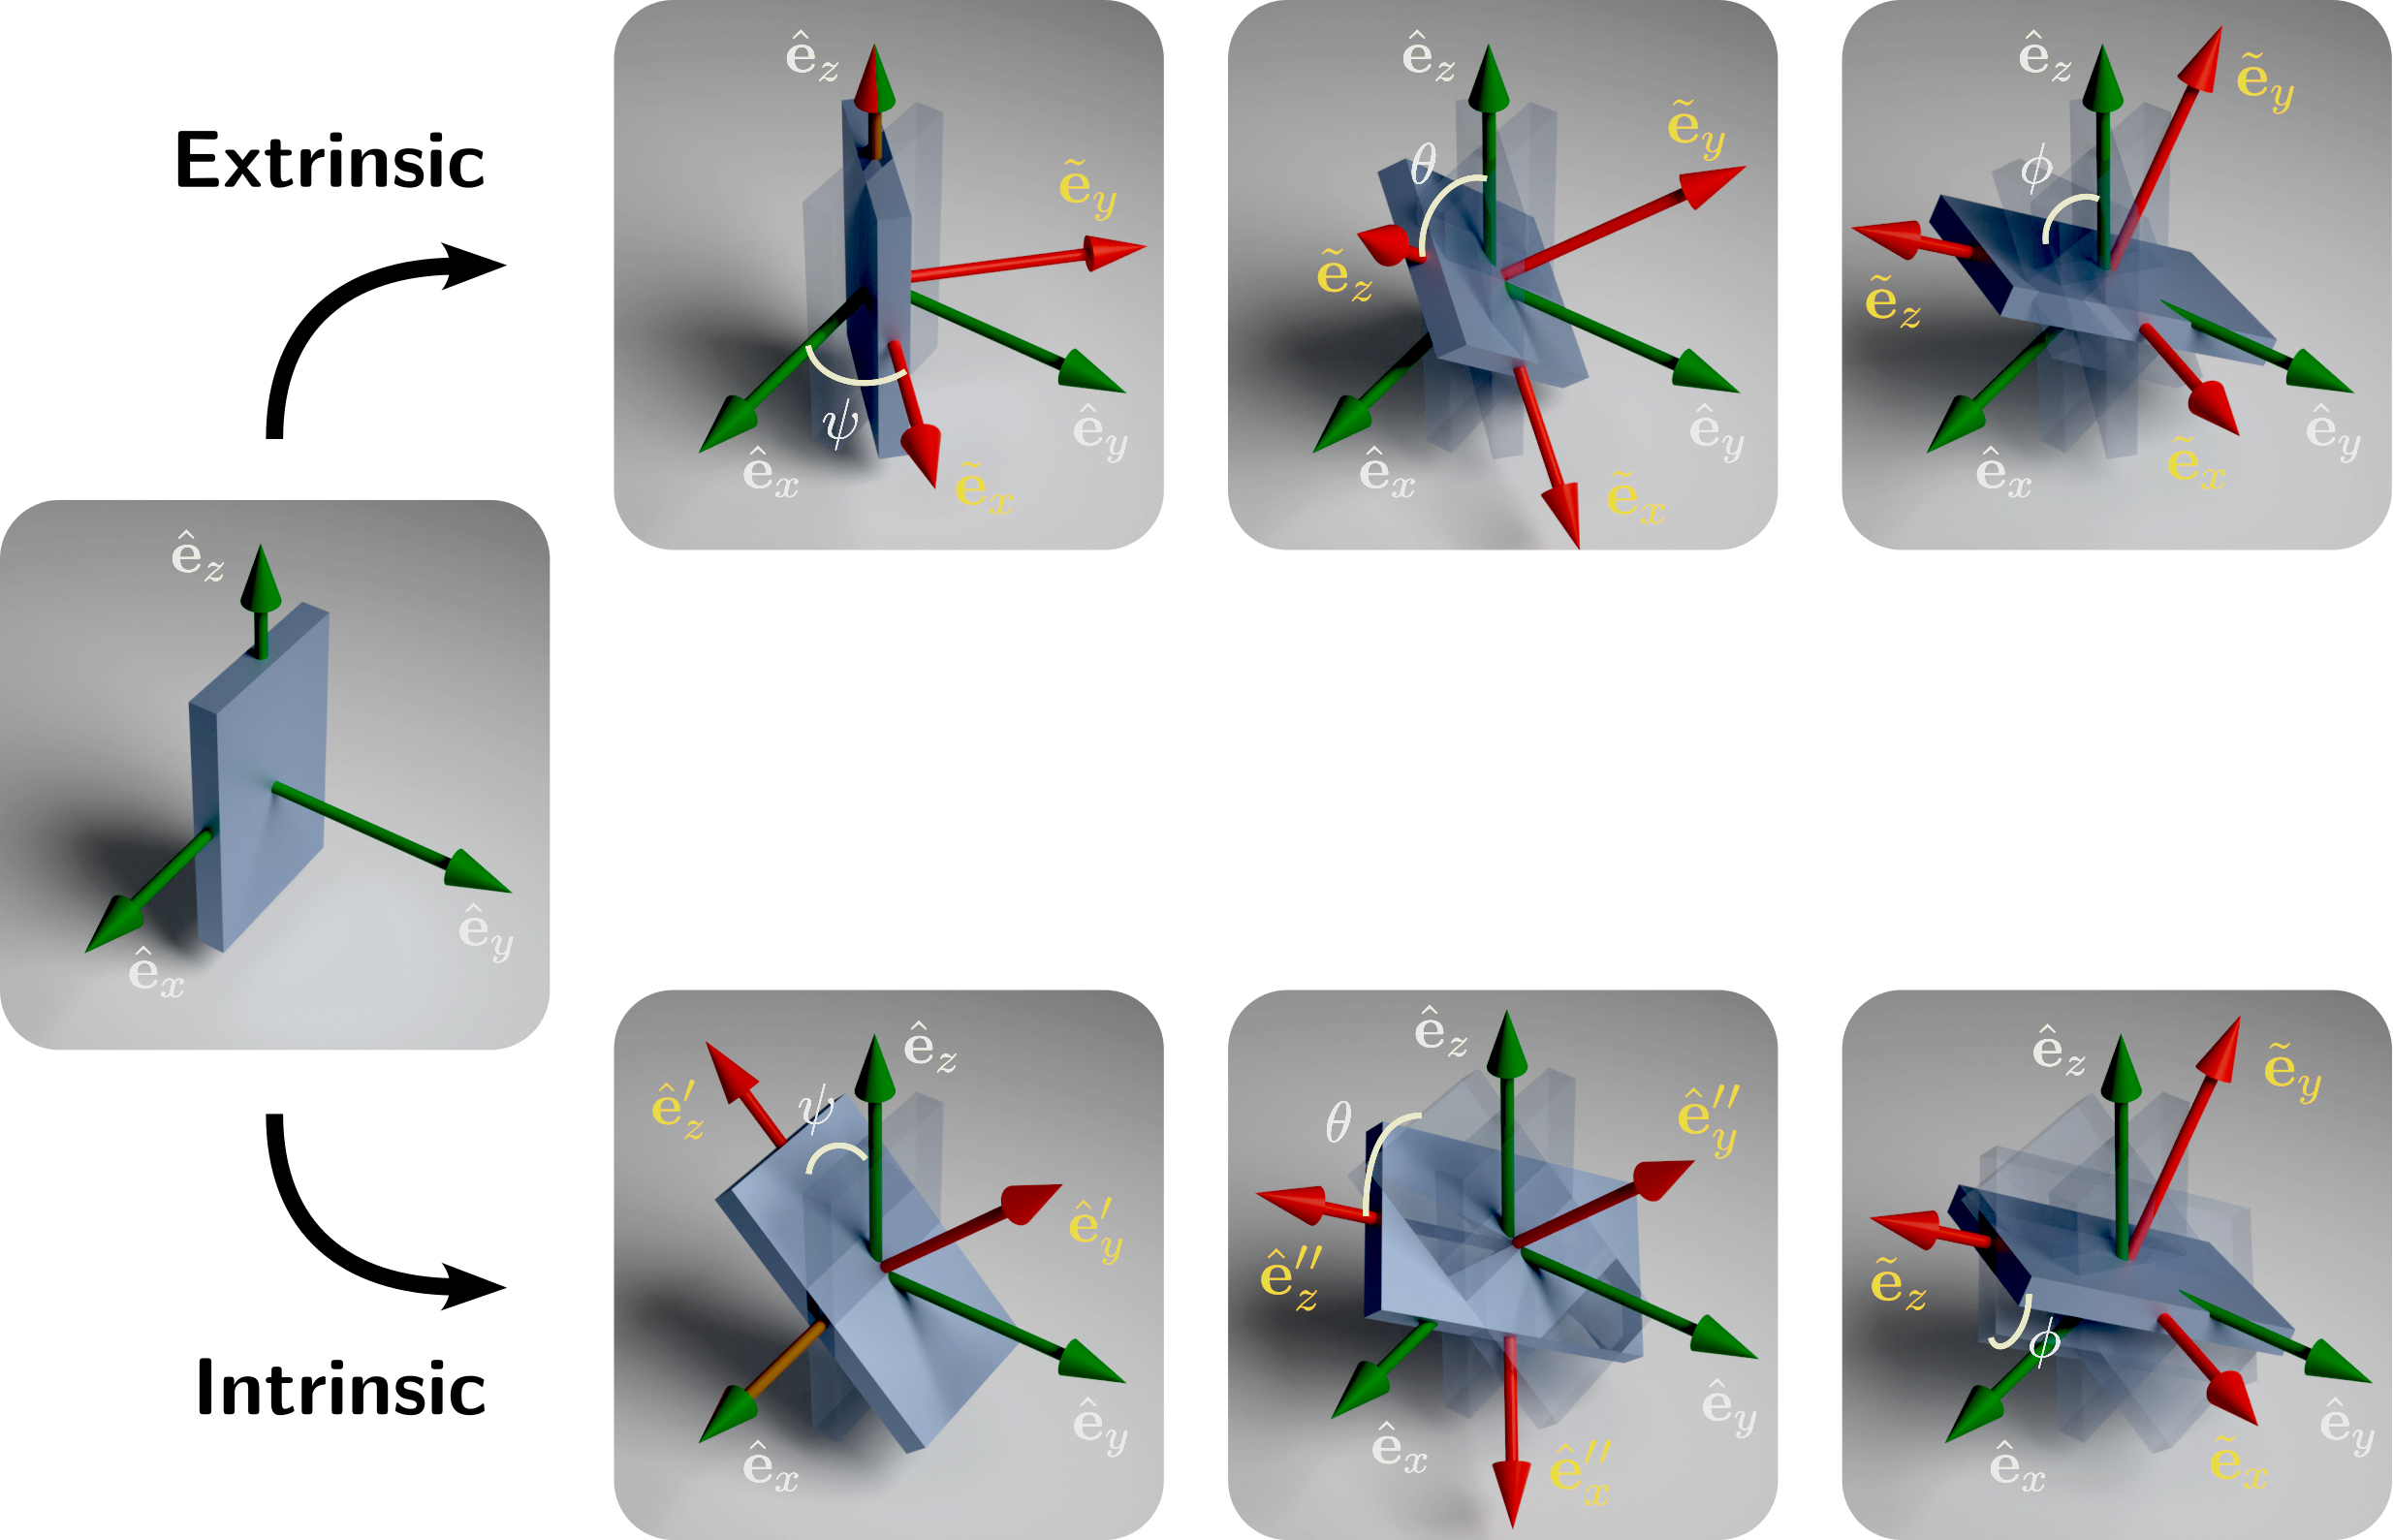
\includegraphics[width=\textwidth]{figs/figExtInt.jpg}
  \caption{Schematic shows 2 ways of performing consecutive rotations to transform from one orientation to the other i.e., extrinsic and intrinsic rotations. Extrinsic rotation is performed about a fixed global axes, while intrinsic rotation about a moving axes that transforms with the object. It is important to note that rotations performed in extrinsic and intrisic form provide the same result (however the order of performing the operation is reversed, as discussed in the main text). Please see the linked \href{https://github.com/sgangaprasath/RotationTut/blob/main/Rotations.ipynb}{\texttt{python}--code} for an example.}
  \label{fig:eulAng3D}
\end{figure}

\subsection{Rotation around \texorpdfstring{$\eh_i$}{eh}}
We will now derive the rotation matrix, $\R_i$ for $i = \{ x, y, z \}$ that performs rotation around different axis, $\eh_i$ when acted on a vector represented in this basis. Fig.~\ref{fig:eulAng3D} shows schematically the effect of this rotation on a rigid object. When $\R_i$ acts on a vector or object, it leaves the component along the $i$-axis fixed while rotating the other two components. In essence, $\R_i$ performs 2D rotation with respect to $i$-axis.
\begin{itemize}
    \item \textbf{Rotation about $\eh_x$}: 
    The rotation matrix about $\eh_x$ by an angle $\psi$, denoted as $\R_x (\psi)$, is given by
    \[
      \R_x(\psi) = 
      \begin{pmatrix} 
    1 & 0 & 0 \\
    0 & \cos(\psi) & -\sin(\psi) \\
    0 & \sin(\psi) & \cos(\psi) 
    \end{pmatrix}.
    \]
    Here positive values of $\psi$ denote rotation in the counter-clockwise direction when looking along $\eh_x$. This is shown schematically as the first step in intrinsic rotation in Fig.~\ref{fig:eulAng3D}.

    \item \textbf{Rotation about $\eh_y$}:
    Rotation about $\eh_y$ by an angle $\theta$ can be performed by the matrix $\R_y(\theta)$ given by
    \[
      \R_y(\theta) =
      \begin{pmatrix} 
    \cos(\theta) & 0 & \sin(\theta) \\
    0 & 1 & 0 \\
    -\sin(\theta) & 0 & \cos(\theta) 
    \end{pmatrix}.
    \]

    \item \textbf{Rotation about $\eh_z$}:
    Rotation about $\eh_z$, denoted as $\R_z(\phi)$, is
    \[
      \R_z(\phi) = 
      \begin{pmatrix} 
    \cos(\phi) & -\sin(\phi) & 0 \\
    \sin(\phi) & \cos(\phi) & 0 \\
    0 & 0 & 1 
    \end{pmatrix}.
    \]
\end{itemize}


\subsubsection*{Sequential rotation of a vector \texorpdfstring{$\v$}{v}}
Consider a vector $\v$ with components in $\eh_i$ coordinate basis $\{ v_1, v_2, v_3 \}$. Performing a sequence of rotations of this vector will modify its orientation but the order of rotation determines the final orientation of $\v$. This is because rotation is intrinsically a non-cummutative operation, which is equivalent to saying that the order of the operation matters. When we rotate $\v$ around $\eh_x$ by $\psi$ followed by rotation around $\eh_y$ by $\theta$ does not necessarily result in rotation around $\eh_y$ by $\theta$ followed around $\eh_x$ by $\psi$. This can be easily seen by the fact that matrix multiplication is not commutative. We can write this sequential operation and the non-cummutivity mathematically as, $\R_x(\psi) \R_y(\theta) \neq \R_y(\theta) \R_x(\psi)$. No two sequences produce the same transformation unless they represent the same rotation.

\subsection{Rotation around arbitrary direction}\label{sec:rodg}
\begin{figure}[t!]
  \centering
  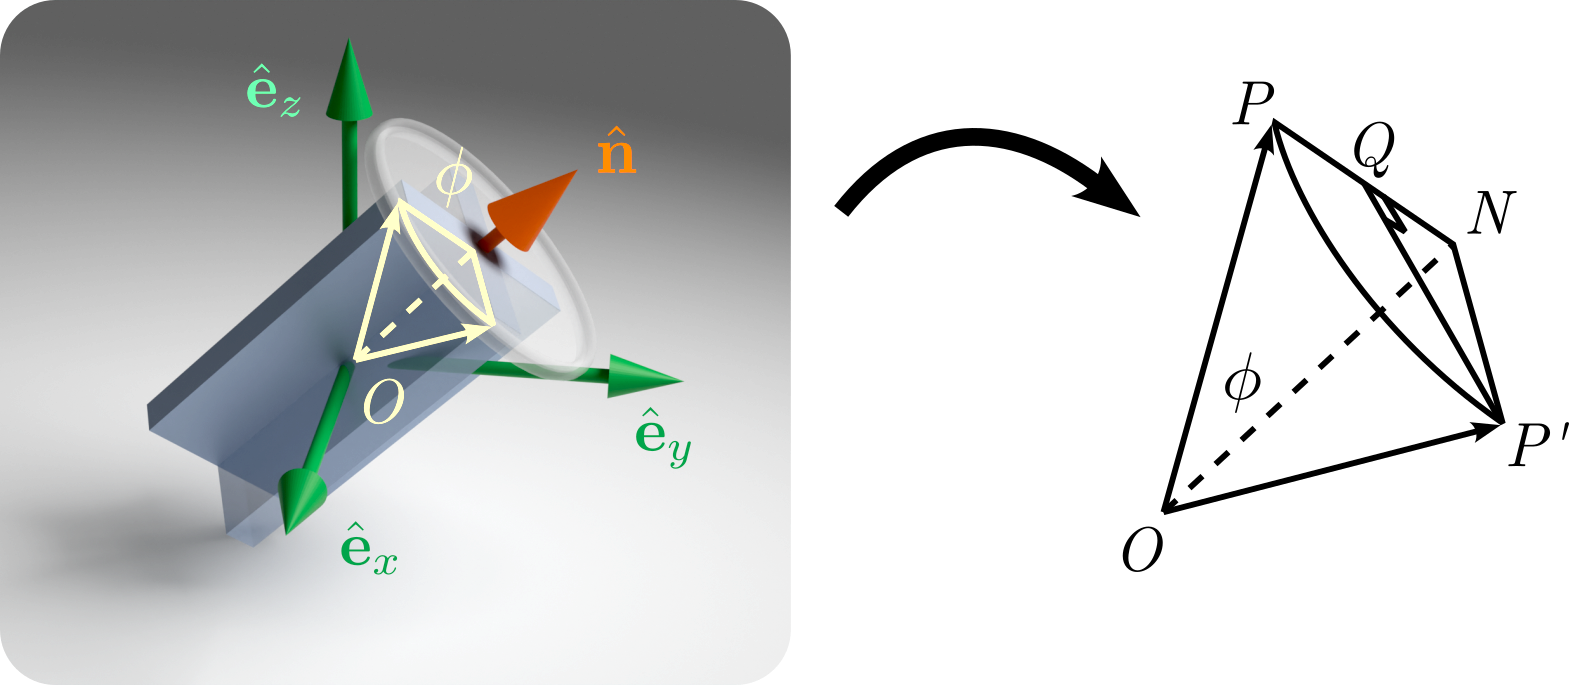
\includegraphics[width=0.75\textwidth]{figs/figRodg.png}
  \caption{Schematic describes the rotation of vector $\v$ represented by $\vec{OP}$ about $\nh$ or $\vec{ON}$ by an angle $\phi$ thereby becoming the new vector $\vt / \vec{OP'}$. This approach is also used to rotate a rigid body as shown here and the matrix to perform such a rotation in Eq.~\ref{eq:rodgForm} is given the name Rodrigues formula.}
  \label{fig:rodg}
\end{figure}
We have seen that simple rotations about $\eh_i$ can be performed by $\R_i$, as it extends 2D rotations. Now we look at how to perform rotation around a specified direction, $\nh$. This not only generalizes rotations around $\eh_i$ but is pivotal for transforming an object's configuration in three-dimensional space.

Let us consider a vector $\v$, shown schematically in Fig.~\ref{fig:rodg}, as $\overrightarrow{OP}$, that is to be rotated around another unit vector $\nh$ along $\overrightarrow{ON}$ by an angle \( \phi \) to reach \( \vt / \overrightarrow{OP'} \). From Fig.~\ref{fig:rodg} we can see that the rotated vector \( \vt \) can be expressed as the sum of three components,
\begin{equation}
     \vt / \overrightarrow{OP'} = \nh + \overrightarrow{NQ} + \overrightarrow{QP'},
\end{equation}
\noindent where \( \overrightarrow{ON} \) is the component of $\v$ along the rotation axis $\nh$, \( \overrightarrow{NQ} \) is the component of \( \overrightarrow{NP'} \)  perpendicular to $\nh$ within the plane containing $\nh$ and $\v$ , and \( \overrightarrow{QP'} \) is the component of \( \overrightarrow{NP'} \) that is perpendicular to $\nh$ and $\v$. It is intuitive to see that the component along the axis, $\nh$ is along $\overrightarrow{ON} = (\v \cdot \nh) \nh$. And the perpendicular component in the plane, $\overrightarrow{NP} = \v - \overrightarrow{ON}$. The rotated perpendicular component is then $\overrightarrow{NQ} = \cos(\phi) \overrightarrow{NP}$. The perpendicular component to the plane ultimately is $\overrightarrow{QP'} = \sin(\phi) (\nh \times \v)$. Summing up these different components then gives the relation between $\v, \nh, \vt$ and $\phi$ as,
\begin{equation}
    \vt  = \cos(\phi) \v + [1 - \cos(\phi)] (\nh \cdot \v) \nh + \sin(\phi) (\nh \times \v).
\end{equation}
This can be reformulated using matrix notation as,
\begin{equation}
\vt = \big[\cos(\phi) \I + (1 - \cos(\phi))\hat{\mathbf{n}}\hat{\mathbf{n}}^\text{T} + \sin(\phi) \bm{\epsilon} \nh \big] \v,
\end{equation}
where \(\I\) is the $3 \times 3$ identity matrix, $\bm{\epsilon} \nh$ is the skew-symmetric matrix corresponding to the vector $\nh$, defined as
\begin{equation}
\bm{\epsilon} \nh = \begin{pmatrix}
0 & -n_3 & n_2 \\
n_3 & 0 & -n_1 \\
-n_2 & n_1 & 0
\end{pmatrix},
\end{equation}
with $\bm{\epsilon} \equiv \epsilon_{ijk}$ being the third order anti-symmetric tensor with the property
\[
  \epsilon_{ijk} = \begin{cases}
    +1 & \ \text{if $(i,j,k)$ are even permutations of (1, 2, 3)}, \\
    -1 & \ \text{if $(i,j,k)$ are odd permutations of (1, 2, 3)}, \\
    0 & \ \text{if $i=j$ or $j=k$ or $i=k$}.
  \end{cases}
\]
and the expression $\bm{\epsilon} \nh = \sum_{k=1}^3 \epsilon_{ijk}n_k$. Thus, the rotation matrix $\R(\phi, \nh)$ is simply
\begin{equation}
\R(\phi, \nh) = \cos(\phi)\I + (1 - \cos(\phi)) \nh \nh^\T + \sin(\phi) \bm{\epsilon} \nh,
\end{equation}
and the rotated vector $\vt$ is obtained simply by acting this matrix on $\v$, i.e., $\vt = \R \v$.

\noindent The unit vector defining the axis of rotation $\hat{\mathbf{n}}$ in $\eh_i$ basis can be written as
\begin{equation}
    \nh = n_1 \eh_x + n_2 \eh_y + n_3 \eh_z,
\end{equation}
with $||\nh||^2 = n_1^2 + n_2^2 + n_3^2 = 1$. The rotation matrix \(\R(\phi, \nh)\) explicitly reads as
\begin{equation}\label{eq:rodgForm}
\R(\phi, \nh) = \begin{pmatrix}
    n_1^2 (1 - \c(\phi)) + \c(\phi) & n_1 n_2 \cdot (1 - \c(\phi)) - n_3 \s(\phi) & n_1 n_3 (1 - \c(\phi)) + n_2 \s(\phi) \\
    n_1 n_2 (1 - \c(\phi)) + n_3 \s(\phi) & n_2^2 (1 - \c(\phi)) + \c(\phi) & - n_1 \s(\phi) + n_2 n_3 (1 - \c(\phi)) \\
    n_1 n_3 (1 - \c(\phi)) - n_2 \s(\phi) & n_1 \s(\phi) + n_2  n_3 \cdot (1 - \c(\phi)) & n_3^2 (1 - \c(\phi)) + \c(\phi)
\end{pmatrix},
\end{equation}
where we have used the short-hand notation $\c(\bullet) \equiv \cos(\bullet), \s(\bullet) \equiv \sin(\bullet)$. This form of $\R(\phi, \nh)$ is sometimes given the name Rodrigues' rotation formula.

\begin{egsBox}[label={egs:rot3Dex1}, float, floatplacement=t]{Rotation using Rodrigues' formula}
  
    \footnotesize
    Consider a scenario where we have a vector $\mathbf{v} = (1, 0, 0)$. Our goal is to rotate this vector by an angle of $\pi/4$ radians around a unit vector $\mathbf{n} = (1, 1, 1)/{\sqrt{3}}$.

    First, we calculate the components of the rotation matrix $\R(\phi, \nh)$ using Rodrigues' formula. With $\phi = {\pi}/{4}$ and $\nh = (1, 1, 1)/{\sqrt{3}}$, the rotation matrix is computed as:

    \[
    \R \Big( \frac{\pi}{4}, \nh \Big) = \frac{1}{2} \begin{pmatrix}
        1+\frac{1}{\sqrt{3}} & 1-\frac{1}{\sqrt{3}} & 1-\frac{1}{\sqrt{3}} \\
        1-\frac{1}{\sqrt{3}} & 1+\frac{1}{\sqrt{3}} & 1-\frac{1}{\sqrt{3}} \\
        1-\frac{1}{\sqrt{3}} & 1-\frac{1}{\sqrt{3}} & 1+\frac{1}{\sqrt{3}}
    \end{pmatrix}.
    \]

    Applying this matrix to the vector $\mathbf{v}$, we find the rotated vector $\vt$ is,
    \[
    \vt = \R \Big( \frac{\pi}{4}, \nh \Big) \mathbf{v} = \frac{1}{2} \begin{pmatrix}
        1+\frac{1}{\sqrt{3}} \\
        1-\frac{1}{\sqrt{3}} \\
        1-\frac{1}{\sqrt{3}}
    \end{pmatrix}.
    \]
    This rotated vector $\vt$ represents the new orientation of $\mathbf{v}$ after the rotation.
\end{egsBox}

\subsection{Extrinsic rotation from \texorpdfstring{$\eh_i$}{ehi} basis to \texorpdfstring{$\et_i$}{eti} basis}\label{sec:ex2int}
In this section we look at one of the most important functions of rotations, which is to transform a coordinate axes from an initial configuration to a target configuration. As we have mentioned briefly earlier and shown schematically in Fig.~\ref{fig:eulAng3D}, rigid objects' orientation or coordinate basis can be transformed from initial to target configuration by either using a global fixed reference frame, referred to as extrinsic rotation or by using the local reference frame which transforms with every rotation operation, referred to as intrinsic form.

We will first look at the more intuitive extrinsic form of rotation between two coordinate basis denoted by $A$, the initial configuration and $B$, the target configuration shown in Fig.~\ref{fig:eulAng3D}. The global coordinate basis is $A$ which is aligned with global axes $\eh_i$ and it must be rotated to reach target frame $B$ with axes $\et_i$. We can do this by performing three rotations: first around the first axis of frame $A$ that is rotation about $\eh_z$, followed by rotation about $\eh_y$ and lastly by rotating about $\eh_x$. As it must be clear, this rotation sequence is performed in the extrinsic form as the global coordinate basis, $\eh_i$ is used for the transformation. It is important to note that this sequence of rotations, starting with the global $z$-axis, followed by the global $y$-axis, and then the global $x$-axis, has equivalent intrinsic rotations. In order to do this in intrinsic form, in Fig.~\ref{fig:eulAng3D} we show that we can traverse from $A$ by first rotating with respect to $\eh_x$ to reach an intermediate frame $A'$ (with axes $\{ \eh'_x, \eh'_y, \eh_z \}$), and second rotation around $\eh'_y$ leading to frame $A''$ (with axes $\{ \eh''_x, \eh''_y, \eh''_z \}$), and third rotation around $\eh''_z$ to arrive at frame $B$.

This particular sequence of rotation starting with the global $z$-axis followed by global $y$-axis then by global $x$-axis is called 321 rotation. The 321 rotation can be represented as composition of rotation matrices, $\R_i$ we have seen in the earlier section. We can perform the rotation about global $z, y, x$-axes by angles $\psi, \theta, \phi$ using product of 3 $\R_i$ matrices given by,
\[
  \R (\psi, \theta, \phi) = \R_x(\phi) \R_y(\theta) \R_z(\psi).
\]

\noindent In the context of 3D rotations, yaw (\( \psi \)), pitch(\( \theta \)), and roll(\( \phi \)) are commonly used terms for 321 rotation sequence,
\[
  \R_{\text{final}} (\psi, \theta, \phi) = 
\begin{pmatrix} 
    \cos(\phi) & -\sin(\phi) & 0 \\
    \sin(\phi) & \cos(\phi) & 0 \\
    0 & 0 & 1 
\end{pmatrix}
\begin{pmatrix}
\cos(\theta) & 0 & \sin(\theta) \\
0 & 1 & 0 \\
-\sin(\theta) & 0 & \cos(\theta)
\end{pmatrix}
\begin{pmatrix} 
    1 & 0 & 0 \\
    0 & \cos(\psi) & -\sin(\psi) \\
    0 & \sin(\psi) & \cos(\psi)
\end{pmatrix}.
\]

\noindent A subtle point worth mentioning is that we have taken some freedom in defining yaw (\( \psi \)), pitch(\( \theta \)), and roll(\( \phi \)) in the case of an extrinsic rotation sequence here, however it is conventionally used in the context of an intrinsic rotation. This results in the following matrix,
\[
  \R_{\text{final}} (\psi, \theta, \phi) = 
\begin{pmatrix}
\c(\psi)\c(\theta) & -\s(\psi)\c(\phi) + \c(\psi)\s(\theta)\s(\phi) & \s(\psi)\s(\phi) + \c(\psi)\s(\theta)\c(\phi) \\
\s(\psi)\c(\theta) & \c(\psi)\c(\phi) + \s(\psi)\s(\theta)\s(\phi) & -\c(\psi)\s(\phi) + \s(\psi)\s(\theta)\c(\phi) \\
-\s(\theta) & \c(\theta)\s(\phi) & \c(\theta)\c(\phi)
\end{pmatrix}.
\]

\begin{egsBox}[label={egs:rot3Dex1}, float, floatplacement=t]{Rotating from initial basis $\eh_i$ to target basis $\et_i$}
  \footnotesize
  Consider a scenario where we need to rotate a coordinate system from an initial basis $\eh_i = \{\eh_x, \eh_y, \eh_z\}$ to a target basis $\et_i = \{\et_x, \et_y, \et_z\}$. Let's assume the rotation involves a yaw of $\dfrac{\pi}{6}$ , a pitch of $\dfrac{\pi}{4}$, and a roll of $\dfrac{\pi}{3}$. Using the 321 rotation sequence, the final rotation matrix is calculated as follows:
 \[
  \R_{\text{final}} (\psi, \theta, \phi) = \begin{pmatrix}
\c(\frac{\pi}{6}) \c(\frac{\pi}{4}) & \s(\frac{\pi}{3}) \s(\frac{\pi}{4}) \c(\frac{\pi}{6}) - \s(\frac{\pi}{6}) \c(\frac{\pi}{3}) & \s(\frac{\pi}{3}) \s(\frac{\pi}{6}) + \s(\frac{\pi}{4}) \c(\frac{\pi}{3}) \c(\frac{\pi}{6}) \\
\s(\frac{\pi}{6}) \c(\frac{\pi}{4}) & \s(\frac{\pi}{3}) \s(\frac{\pi}{6}) \c(\frac{\pi}{4}) + \c(\frac{\pi}{3}) \c(\frac{\pi}{6}) & \s(\frac{\pi}{6}) \s(\frac{\pi}{4}) \c(\frac{\pi}{3}) - \s(\frac{\pi}{3}) \c(\frac{\pi}{6}) \\
-\s(\frac{\pi}{4}) & \s(\frac{\pi}{3}) \c(\frac{\pi}{4}) & \c(\frac{\pi}{3}) \c(\frac{\pi}{4})
\end{pmatrix}.
\]

 This matrix represents the combined effect of yaw, pitch, and roll rotations, transforming the initial basis $\eh_i$ to the target basis $\et_i$. The columns of this rotation matrix can be interpreted as follows:
  \begin{itemize}
    \item The first column represents the target basis vector $\et_x$ written in terms of the initial basis vectors $\eh_i$.
    \item The second column represents the target basis vector $\et_y$ written in terms of the initial basis vectors $\eh_i$.
    \item The third column represents the target basis vector $\et_z$ written in terms of the initial basis vectors $\eh_i$.
  \end{itemize}
\end{egsBox}

\subsubsection*{313 Rotation Sequence}
Just like we can transform between $\eh_i$ to $\et_i$ via 321 rotations, we can do this transformation via 11 other sequences (which we will discuss soon). Another such sequence is the 313 rotation sequence for which the rotation matrix $\R$ is the product of rotations about $\eh_z$, followed by $\eh_x$, and again $\eh_z$. The rotation matrix  $\R$ for the 313 sequence is given by,
\[
  \R (\psi, \theta, \phi) = \R_z(\psi) \R_x(\theta) \R_z(\phi),
\]
where \( \R_z(\psi) \) and \( \R_z(\phi) \) are the rotation matrices about the $z$-axis, and \( \R_x(\theta) \) is the rotation matrix about the $x$-axis. 

\noindent The final rotation matrix \( \R_{\text{final}} (\psi, \theta, \phi) \) for the 313 rotation sequence can be written as,
\[
\R_{\text{final}} (\psi, \theta, \phi) = \begin{pmatrix}
-\s(\phi)\s(\psi)\c(\theta) + \c(\phi)\c(\psi) & -\s(\phi)\c(\psi) - \s(\psi)\c(\phi)\c(\theta) & \s(\psi)\s(\theta) \\
\s(\phi)\c(\psi)\c(\theta) + \s(\psi)\c(\phi) & -\s(\phi)\s(\psi) + \c(\phi)\c(\psi)\c(\theta) & -\s(\theta)\c(\psi) \\
\s(\phi)\s(\theta) & \s(\theta)\c(\phi) & \c(\theta)
\end{pmatrix}.
\]

\noindent In three-dimensional space, like the 321, 313 rotation sequence we have seen above, Euler angle rotations can be represented via a total of 12 distinct sequences. These sequences are derived from permutations of rotations about the three principal axes, $\eh_i$. For each sequence, the first and last rotations must be about different axes, and the middle rotation is about the axis not used in the first rotation. This rule leads to 12 unique combinations: 321, 323, 313, 312, 231, 213, 212, 232, 123, 132, 121, 131.

We have seen so far that the rotation between two different coordinate basis $\eh_i$ and $\et_i$ can be achieved either by using Rodrigues' formula with $\nh, \phi$ in Eq.~\ref{eq:rodgForm} or through 3 Euler angles, $\{\psi, \theta, \phi\}$. In the former case of it might seem as though we require 4--degrees of freedom, $\{ n_i, \phi \}$, the unit-vector constraint of $\nh$ i.e. $||\nh||^2 = 1$, however, reduces the required variables to 3. The attached \href{https://github.com/sgangaprasath/RotationTut/blob/main/Rotations.ipynb}{\texttt{python}--code} has details of such an implementation.

\subsubsection*{Connection between extrinsic and intrinsic transformations}

We have seen that in the extrinsic form, each rotation is performed with respect to a fixed coordinate basis, $\eh_i$. These rotations are easier to visualize as they relate to a stationary frame of reference. In contrast, intrinsic rotations in Fig.~\ref{fig:eulAng3D} are performed with respect to the rotating coordinate system. The key to connection between extrinsic and intrinsic transformations lies in the order of applied rotations. An extrinsic rotation sequence can be converted to an intrinsic sequence by reversing the order of rotations and vice versa. This is because rotating an object first about one axis and then about another in a fixed coordinate system (extrinsic) is equivalent to rotating it about the second axis and then the first in its own coordinate system (intrinsic).

For example, an extrinsic rotation sequence about the 123 ($\eh_x \rightarrow \eh_y \rightarrow \eh_z$) is equivalent to an intrinsic rotation sequence 321 ($\eh_z \rightarrow \eh'_y \rightarrow \eh''_x$). Though the order of applied sequence is reversed, the rotation matrix for both these sequences is the same. This relationship allows for the translation of a series of rotations from one perspective to another. In order to gain a deeper understanding of this connection, we refer the reader to this \href{https://dominicplein.medium.com/extrinsic-intrinsic-rotation-do-i-multiply-from-right-or-left-357c38c1abfd}{link}.

\subsubsection*{Vector components in different coordinate basis}
In sec.~\ref{sec:VecComp2D} we saw that the vector components in 2D transform under the rule, $\v = \Q^\T \vt$ and $\vt = \Q \v$. This transformation is valid also in 3D where the matrix $\Q = \{ \et_x, \et_y, \et_z \}$, which can be written explicitly as
\[
  \Q  =
  \begin{pmatrix} 
  \etx \cdot \ehx & \etx \cdot \ehy & \etx \cdot \ehz\\
  \ety \cdot \ehx & \ety\cdot \ehy & \ety\cdot \ehz\\
  \etz \cdot \ehx & \etz\cdot \ehy & \etz\cdot \ehz
  \end{pmatrix}.
\]
Let us consider three basis vectors $\ehx, \ehy, \ehz$ pointing along the $x, y, z$-axis respectively. Similar to our 2D calculations, When the vectors $\ehx, \ehy$ are rotated by an angle $\phi$ in the counter-clockwise direction around the $\ehz$ axis, they give rise to $\etx, \ety$. It is straightforward to see that $\ehx\cdot\etx=\ehy\cdot\ety=\cos \phi$ and $\ehy\cdot\etx = -\ehx\cdot\ety = \sin \phi$. The third basis vector $\ehz$ remains unchanged during this rotation, so $\ehz\cdot\etz = 1$. The rotation tensor $\Q$ in 3D then reduces to
\[
  \Q  = 
  \begin{pmatrix} 
  \cos \phi & \sin \phi & 0 \\
  -\sin \phi & \cos \phi & 0 \\
  0 & 0 & 1
  \end{pmatrix}.
\]
\noindent Now, a vector $\v$ with components $\{ v_1, v_2, v_3 \}$ in the $\eh_i$ basis can be transformed to components $\{ \vts_1, \vts_2, \vts_3 \}$ in the rotated basis $\et_i$ using $\vt = \Q \v$  and the inverse operation can be done using  $\v = \Q^\T \vt$. The \texttt{python}--code for an implementation of this to transform the basis vectors is available \href{https://github.com/sgangaprasath/RotationTut/blob/main/Rotations.ipynb}{here}.

\subsubsection*{Properties of rotation matrix in 3D}
Apart from orthonormal property of rotation matrix (which is valid also in 3D), $\R$ has the following properties:
\begin{itemize}
  \item A 3D rotation matrix \(\R\) is an orthonormal matrix, meaning \(\R^\T \R = \R \R^\T = \I\), where \(\R^\T\) is the transpose of \(\R\) and \(\I\) is the identity matrix(\(\R^{-1} = \R^\T\).). The determinant of \(\R\) in the special orthogonal group SO(3) is +1, indicating that the rotation preserves the orientation of a right-handed coordinate system: \(\det(\R) = +1\).
  \item The set of all orthonormal matrices with determinant +1 forms the special orthogonal group SO(3).
  \item A 3D rotation matrix always has one real eigenvalue, which is +1, with the corresponding eigenvector being the axis of rotation. The other two eigenvalues are complex conjugates of each other and lie on the unit circle in the complex plane.
  \item Every orthonormal matrix in 3D corresponds to rotation about a specific axis by a certain angle, known as the axis-angle representation. The rotation axis, $\nh$ is the eigenvector associated with the eigenvalue +1 of the matrix, and the rotation angle \(\phi\) can be calculated from the matrix's trace: \(\phi = \arccos\Big[ \dfrac{\text{tr}(\R) - 1}{2} \Big]\).
\end{itemize}
\subsection{Gimbal lock}
\begin{figure}[t!]
  \centering
  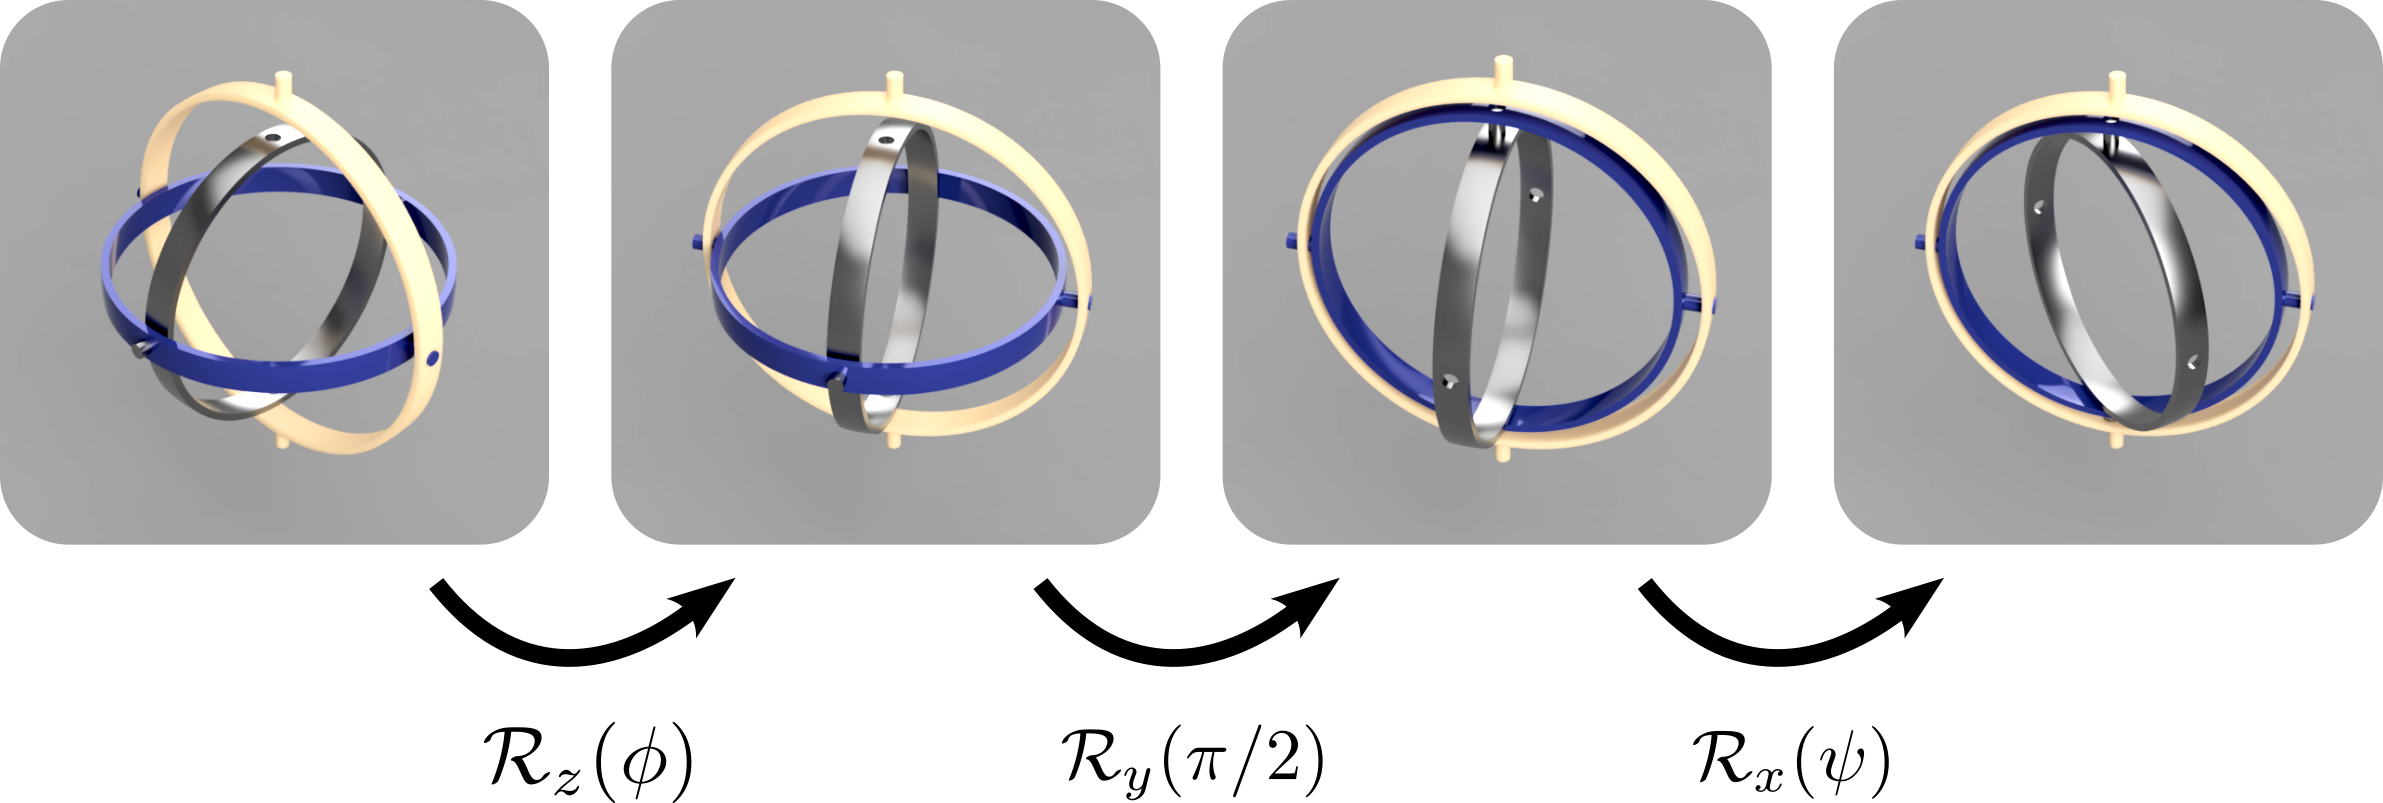
\includegraphics[width=\textwidth]{figs/figGimbal.png}
  \caption{Schematic showing the phenomenon of Gimbal locking occuring given the initial configuration is transformed by the 321 rotation sequence. Such a locking situation arises when rotating the axis, $\eh_i$ by $\R_z(\phi)$ followed by $\R_y(\pi/2)$ then by $\R_x(\psi)$. It is worth noting that Gimbal locking occurs with all the 12 Euler angle sequences discussed in sec.~\ref{sec:ex2int}.}
  \label{fig:gimbLck}
\end{figure}
Gimbal is a structure used to provide pivoted support to an object so that the object can be oriented in any specified direction (see Fig.~\ref{fig:gimbLck}). Gimbal lock is a phenomenon in which the connection of the rings pointing towards three directions lose a degree-of-freedom as two rings align themselves. This can occur in a sequence of rotations where one rotation leads to an alignment of two axes. For example, in a yaw-pitch-roll system (321-rotation sequence) shown in , if the pitch angle (\( \theta \)) is rotated by \( \pm 90^\circ \), the yaw and the roll axes align. This alignment causes the loss of one degree of freedom, making it impossible to distinguish between yaw and roll motions.
\[
\R_{\text{final}} (\psi, \theta, \phi) = 
\begin{pmatrix}
1 & 0 & 0 \\
0 & \c(\phi) & -\s(\phi) \\
0 & \s(\phi) & \c(\phi)
\end{pmatrix}
\begin{pmatrix}
\c(\theta) & 0 & \s(\theta) \\
0 & 1 & 0 \\
-\s(\theta) & 0 & \c(\theta)
\end{pmatrix}
\begin{pmatrix}
\c(\psi) & -\s(\psi) & 0 \\
\s(\psi) & \c(\psi) & 0 \\
0 & 0 & 1
\end{pmatrix}.
\]

\noindent When \(\theta = 90^\circ\) or \(\theta = \dfrac{\pi}{2}\) radians, the pitch rotation matrix simplifies to,
\[
\R_{y}(\pi/2) = 
\begin{pmatrix}
0 & 0 & 1 \\
0 & 1 & 0 \\
-1 & 0 & 0
\end{pmatrix}.
\]
Multiplying these matrices together with \(\theta = 90^\circ\), we get the final rotation matrix as,
\begin{align}
\R_{\text{final}} (\psi, \pi/2, \phi) = \R_{x}(\psi) \R_{y}(\pi/2) \R_{z}(\phi) = 
\begin{pmatrix}
0 & 0 & 1 \\
\s(\psi + \phi) & \c(\psi + \phi) & 0 \\
-\c(\psi + \phi) & \s(\psi + \phi) & 0
\end{pmatrix}. \label{eq:gimbEq}
\end{align}
This matrix shows that the rotation about the third axis is now the only distinct motion. The rotation about the yaw and roll axes ($\eh_z$ and $\eh_x$) becomes dependent on each other, represented by the combination of \(\psi\) and \(\phi\) in the second and third rows. Essentially when \(\theta = \pi/2\), the yaw (\(\psi\)) and roll (\(\phi\)) rotations combine, resulting in the loss of one degree of freedom. This is the phenomenon of gimbal lock, where the system cannot differentiate between yaw and roll rotations independently. Though we see that Gimbal lock is an issue seen in a Gimbal parameterised using Euler angles, it points to a fundamental issue with Euler angle representation of rotation. We see in Eq.~\ref{eq:gimbEq} that we can no more distinguish between change in $\psi$ or $\phi$ but rather only $(\psi + \phi)$. This happens to all rotation matrices, $\R$ parameterised with Euler angles at particular values of $\psi$ or $\theta$ or $\phi$.

The implications of gimbal lock are significant in fields that rely on precise 3D rotations, such as aerospace and robotics. In these fields, gimbal lock can lead to unpredictable behavior and loss of control. For instance, in an aircraft, if gimbal lock occurs, the pilot may lose the ability to control the aircraft's orientation accurately. One common method to overcome gimbal lock is to use a different representation for 3D rotations, such as quaternions. Quaternions do not suffer from gimbal lock because they represent rotations in four dimensions, avoiding the alignment issue inherent in three-dimensional Euler angles which we shall elucidate in the next section.

\section{Quaternion}\label{sec:quat}
We have so far seen two forms of rotations, one using complex numbers in 2D and the standard matrix form acting on vectors in 2D and 3D. In this last section, we will see how to extend the ideas of complex numbers from 2D into 3D using quaternions. Quaternions form an interesting algebra, which is beyond the scope of this primer, nevertheless, the interested reader can look at \cite{hanson2005visualizing, vince2008geometric} for detailed discussions.

Quaternions are an extension of complex numbers, represented with one real part and three imaginary parts. A quaternion $q$ is expressed as,
\begin{equation*}
    q = q_0 + q_1i + q_2j + q_3k,
\end{equation*}
where $q_i \in \Rn$ for $i=\{0, \dots, 3 \}$, and \( i, j, k \) are the fundamental quaternion units. These units, similar to the imaginary constant in complex numbers, have specific multiplication rules that are crucial to their behaviour. They are,
\begin{align*}
    i^2 &= j^2 = k^2 = ijk = -1 ,\\
    ij &= k, \quad ji = -k, \\
    jk &= i, \quad kj = -i, \\
    ki &= j, \quad ik = -j.
\end{align*}
The non-commutative nature of quaternion multiplication (e.g., \( ij \neq ji \)) is a key feature that distinguishes them from complex numbers and allows for their unique application. Quaternions are also represented in 4--vector form as $q = \{ q_0, \q \}$ where $\q$ is a vector in 3D with components $\q = \{ q_1, q_2, q_3 \}$.
Quaternion multiplication is a key operation that combines the effects of two rotations. Given two quaternions \( p = p_0 + p_1i + p_2j + p_3k \) and \( q = q_0 + q_1i + q_2j + q_3k \), their product \( p \star q \) is not commutative and can be expressed as
\begin{align}
  p \star q =\ & (p_0 q_0 - p_1 q_1 - p_2 q_2 - p_3 q_3) + \nonumber \\
         & (p_0 q_1 + p_1 q_0 + p_2 q_3 - p_3 q_2)i + \nonumber \\
         & (p_0 q_2 - p_1 q_3 + p_2 q_0 + p_3 q_1)j + \nonumber \\
         & (p_0 q_3 + p_1 q_2 - p_2 q_1 + p_3 q_0)k. \label{eq:quatMul}
\end{align}
\noindent This result can be rearranged into a matrix multiplication form, often used in numerical implementations, where the quaternion is represented as a \( 4 \times 1 \) column vector, and the coefficients form a \( 4 \times 4 \) matrix. The matrix representation of the quaternion multiplication is given by, 
\[
\begin{pmatrix}
p_0 & -p_1 & -p_2 & -p_3 \\
p_1 & p_0 & -p_3 & p_2 \\
p_2 & p_3 & p_0 & -p_1 \\
p_3 & -p_2 & p_1 & p_0 
\end{pmatrix}
\begin{pmatrix}
q_0 \\
q_1 \\
q_2 \\
q_3
\end{pmatrix}
=
\begin{pmatrix}
p_0 q_0 - p_1 q_1 - p_2 q_2 - p_3 q_3 \\
p_0 q_1 + p_1 q_0 + p_2 q_3 - p_3 q_2 \\
p_0 q_2 - p_1 q_3 + p_2 q_0 + p_3 q_1 \\
p_0 q_3 + p_1 q_2 - p_2 q_1 + p_3 q_0
\end{pmatrix}.
\]
\noindent We can write this multiplication operation in terms of vector operations as $p \star q = (p_0q_0 - \p \cdot \q, p_0 \q + q_0 \p + \p \times \q)$. Here $\cdot$, $\times$ operations are the standard dot--product and cross--product used for 3--vectors. Quaternions also have conjugates, $\bar{\q} = \{q_0, -q_1, -q_2, -q_3\}$, similar to complex numbers, and with this the multiplication becomes, $q \star \bar{q} = \{ q \cdot q, 0 , 0 , 0\} = \{ q_0^2 + \q \cdot \q, 0, 0, 0 \} = \{\sum_{i=0}^3 q_i^2, 0, 0, 0\}$.

\subsection{Rotation about arbitrary direction}
In order to capture rotation with quaternions, we first restrict them to be of unit magnitude, i.e. $q \star \bar{q} = 1$. Then we define the axis of rotation using quaternions and construct the rotation quaternion, followed by the action on the vector that must be rotated.

Let the unit vector denoting the axis of rotation be $\nh = n_i \eh_i$ with $\nh \cdot \nh = \sum_{i=1}^3 n_i^2 = 1$ and the rotation quaternion, $q = q_0 + q_1i + q_2j + q_3k$ be defined as,
\begin{align*}
    q_0 &= \cos\left(\frac{\phi}{2}\right), \\
    q_1 &= n_1 \sin\left(\frac{\phi}{2}\right), \\
    q_2 &= n_2 \sin\left(\frac{\phi}{2}\right), \\
    q_3 &= n_3 \sin\left(\frac{\phi}{2}\right),
\end{align*}
where $\phi$ is the angle of rotation. We can write this rotation quaternion compactly in 4--vector form as $q = \{ \cos (\phi/2), \nh \sin(\phi/2) \}$. With this definition, the Rodrigues' formula for rotation matrix, $\R(\phi,\nh)$ around $\nh$ by an angle $\phi$ in Eq.~\ref{eq:rodgForm} can be written in terms of rotation quaternion components, \( q_0, q_1, q_2, \) and \( q_3 \) as,
\begin{equation}
\R(q) \equiv \R(\phi, \nh) = \begin{pmatrix}
    q_0^2 + q_1^2 - q_2^2 - q_3^2 & 2(q_1q_2 - q_0q_3) & 2(q_1q_3 + q_0q_2) \\
    2(q_1q_2 + q_0q_3) & q_0^2 - q_1^2 + q_2^2 - q_3^2 & 2(q_2q_3 - q_0q_1) \\
    2(q_1q_3 - q_0q_2) & 2(q_2q_3 + q_0q_1) & q_0^2 - q_1^2 - q_2^2 + q_3^2
\end{pmatrix}.
\end{equation}

\subsubsection*{Rotation of a vector}
Given a vector $\v$, we know from sec.~\ref{sec:rodg} that we can rotate a vector by an angle $\phi$ by constructing $\R(\phi, \nh)$ and obtained the transformed vector by simply performing the matrix multiplication operation, $\vt = \R(\phi, \nh) \v$. However, in order to rotate a vector $\v$ using quaternions, we need to construct two quaternions: $(i)$ rotation quaternion, $q = \{ \cos (\phi/2), \nh \sin(\phi/2) \}$, $(ii)$ 4--vector form of $\v$ i.e. $p = \{0, \v\}$ (a pure quaternion, with vanishing first component i.e. $p_0=0$). The rotation operation is then simply, $(q \star p \star \bar{q})$. This can be expanded explicitly as
\[
  \tilde{p} = q \star \{ 0, \v \} \star \bar{q} = \{ 0, \R(q) \v \},
\]
where the quaternion multiplication rule in Eq.~\ref{eq:quatMul} is used and $\tilde{p} = \{ 0, \vt \} $.

\subsubsection*{Connecting Euler angles}
We have seen that the rotation matrix, $\R (\phi, \nh)$ can be mapped to a quaternion $q = \{ \cos (\phi/2), \nh \sin (\phi/2) \}$. We can also do a similar transformation from Euler angle rotation $\R (\psi, \theta, \phi)$ to quaternion by first choosing the rotation sequence and then describe the rotation using a quaternion. Let us say we would like to follow 313 sequence, $R_{313}(\psi, \theta, \phi)$ can be written as quaternion $q$ with components,
\begin{align*}
  q_0 =& \ \cos \Big( \frac{\theta}{2} \Big) \cos \frac{1}{2} \Big( \psi + \phi \Big), \\
  q_1 =& \ \sin \Big( \frac{\theta}{2} \Big) \sin \frac{1}{2} \Big( \phi - \psi \Big), \\
  q_2 =& \ \sin \Big( \frac{\theta}{2} \Big) \cos \frac{1}{2} \Big( \phi - \psi \Big), \\
  q_3 =& \ \cos \Big( \frac{\theta}{2} \Big) \sin \frac{1}{2} \Big( \psi + \phi \Big).
\end{align*}

\subsection{Extension of complex numbers}
As we have mentioned earlier, quaternions generalize complex numbers from 2D to 3D. In order to see this in action, we can write the rotation quaternion as $q = \exp (\{0, \nh \phi/2 \})$. With this definition, we can see that the exponential of a pure quaternion (of unit modulus) satisfies,
\[
  \exp ( \{ 0, \nh \phi/2 \}) = \cos(\phi/2) + \nh \sin(\phi/2).
\]
One easy way to check the validity is to set $\nh = \{ 1, 0, 0 \}$ and see that the expression reduces to the standard complex number, $q = \cos (\phi/2) + i \sin (\phi/2)$.

\noindent Continuing, we have seen in sec.~\ref{sec:comp2d} that multiplying two complex numbers is simpler in the polar form. Multiplying quaternions in polar form follows a similar behaviour. Consider two quaternions in polar form, $p = \{ r_1, \nh_1 \phi_1/2 \}, q = \{ r_2, \nh_2 \phi_2/2 \}$, then the multiplication rule is simply,
\[
  p \star q = \{ r_1, \nh_1 \phi_1/2 \} \star \{ r_2, \nh_2 \phi_2/2 \} = \{ r_1 r_2, \mh \phi_{12}/2 \},
\]
where $\cos (\phi_{12}/2) = p_0q_0 - \p \cdot \q$ and
\[
  \mh = \frac{p_0 \q + q_0 \p + \p \times \q}{||p_0 \q + q_0 \p + \p \times \q||}.
\]
It is easy to verify that $p \star q$ reduces to Eq.~\ref{eq:compMult} when $\nh_1 = \nh_2 = \{ 1, 0, 0 \}$.

\subsubsection*{Properties of quaternions}
Quaternions are a compact way to represent rotations as one needs only 4 components of $q$ instead of 9 components of $\R$. Further, all unit quaternions represent rotation and captures a space of S(3) representing a 3--sphere. Unlike Euler angle form of parameterising rotation matrix, $\R$ the unit quaternion, $q$ avoids Gimbal locking because there are no singularities associated with them. This has been leveraged for interpolation in animation for camera movement. Nevertheless, quaternions are complex mathematically and are less intuitive in terms of what the values represent as they must be converted to $\phi, \nh$ to gain insights.

\section{Conclusion}

In summary, we have seen in this primer some of the properties of rotation in 2D and 3D with examples. We have seen how to rotate vectors, coordinate basis, and rigid objects. Finally, we introduced quaternions which are a compact way of representing rotations in 3D. The \href{https://github.com/sgangaprasath/RotationTut/blob/main/Rotations.ipynb}{\texttt{python}--code} accompanying this primer has the numerical implementation of the various methods discussed here. In the second part of this primer, we will extend ideas from this primer to curves. Rotations are intimately tied to curvature and twist about which we will explore in detail there.

\bibliographystyle{plain}
\bibliography{reference.bib}

\end{document}